%% ODER: format ==         = "\mathrel{==}"
%% ODER: format /=         = "\neq "
%
%
\makeatletter
\@ifundefined{lhs2tex.lhs2tex.sty.read}%
  {\@namedef{lhs2tex.lhs2tex.sty.read}{}%
   \newcommand\SkipToFmtEnd{}%
   \newcommand\EndFmtInput{}%
   \long\def\SkipToFmtEnd#1\EndFmtInput{}%
  }\SkipToFmtEnd

\newcommand\ReadOnlyOnce[1]{\@ifundefined{#1}{\@namedef{#1}{}}\SkipToFmtEnd}
\DeclareFontFamily{OT1}{cmtex}{}
\DeclareFontShape{OT1}{cmtex}{m}{n}
  {<5><6><7><8>cmtex8
   <9>cmtex9
   <10><10.95><12><14.4><17.28><20.74><24.88>cmtex10}{}
\DeclareFontShape{OT1}{cmtex}{m}{it}
  {<-> ssub * cmtt/m/it}{}
\newcommand{\texfamily}{\fontfamily{cmtex}\selectfont}
\DeclareFontShape{OT1}{cmtt}{bx}{n}
  {<5><6><7><8>cmtt8
   <9>cmbtt9
   <10><10.95><12><14.4><17.28><20.74><24.88>cmbtt10}{}
\DeclareFontShape{OT1}{cmtex}{bx}{n}
  {<-> ssub * cmtt/bx/n}{}
\newcommand{\tex}[1]{\text{\texfamily#1}}	% NEU

\newcommand{\Sp}{\hskip.33334em\relax}


\newcommand{\Conid}[1]{\mathit{#1}}
\newcommand{\Varid}[1]{\mathit{#1}}
\newcommand{\anonymous}{\kern0.06em \vbox{\hrule\@width.5em}}
\newcommand{\plus}{\mathbin{+\!\!\!+}}
\newcommand{\bind}{\mathbin{>\!\!\!>\mkern-6.7mu=}}
\newcommand{\rbind}{\mathbin{=\mkern-6.7mu<\!\!\!<}}% suggested by Neil Mitchell
\newcommand{\sequ}{\mathbin{>\!\!\!>}}
\renewcommand{\leq}{\leqslant}
\renewcommand{\geq}{\geqslant}

%mathindent has to be defined
\@ifundefined{mathindent}%
  {\newdimen\mathindent\mathindent\leftmargini}%
  {}%

\def\resethooks{%
  \global\let\SaveRestoreHook\empty
  \global\let\ColumnHook\empty}
\newcommand*{\savecolumns}[1][default]%
  {\g@addto@macro\SaveRestoreHook{\savecolumns[#1]}}
\newcommand*{\restorecolumns}[1][default]%
  {\g@addto@macro\SaveRestoreHook{\restorecolumns[#1]}}
\newcommand*{\aligncolumn}[2]%
  {\g@addto@macro\ColumnHook{\column{#1}{#2}}}

\resethooks

\newcommand{\onelinecommentchars}{\quad-{}- }
\newcommand{\commentbeginchars}{\enskip\{-}
\newcommand{\commentendchars}{-\}\enskip}

\newcommand{\visiblecomments}{%
  \let\onelinecomment=\onelinecommentchars
  \let\commentbegin=\commentbeginchars
  \let\commentend=\commentendchars}

\newcommand{\invisiblecomments}{%
  \let\onelinecomment=\empty
  \let\commentbegin=\empty
  \let\commentend=\empty}

\visiblecomments

\newlength{\blanklineskip}
\setlength{\blanklineskip}{0.66084ex}

\newcommand{\hsindent}[1]{\quad}% default is fixed indentation
\let\hspre\empty
\let\hspost\empty
\newcommand{\NB}{\textbf{NB}}
\newcommand{\Todo}[1]{$\langle$\textbf{To do:}~#1$\rangle$}

\EndFmtInput
\makeatother
%
%
%
%
%
%
% This package provides two environments suitable to take the place
% of hscode, called "plainhscode" and "arrayhscode". 
%
% The plain environment surrounds each code block by vertical space,
% and it uses \abovedisplayskip and \belowdisplayskip to get spacing
% similar to formulas. Note that if these dimensions are changed,
% the spacing around displayed math formulas changes as well.
% All code is indented using \leftskip.
%
% Changed 19.08.2004 to reflect changes in colorcode. Should work with
% CodeGroup.sty.
%
\ReadOnlyOnce{polycode.fmt}%
\makeatletter

\newcommand{\hsnewpar}[1]%
  {{\parskip=0pt\parindent=0pt\par\vskip #1\noindent}}

% can be used, for instance, to redefine the code size, by setting the
% command to \small or something alike
\newcommand{\hscodestyle}{}

% The command \sethscode can be used to switch the code formatting
% behaviour by mapping the hscode environment in the subst directive
% to a new LaTeX environment.

\newcommand{\sethscode}[1]%
  {\expandafter\let\expandafter\hscode\csname #1\endcsname
   \expandafter\let\expandafter\endhscode\csname end#1\endcsname}

% "compatibility" mode restores the non-polycode.fmt layout.

\newenvironment{compathscode}%
  {\par\noindent
   \advance\leftskip\mathindent
   \hscodestyle
   \let\\=\@normalcr
   \let\hspre\(\let\hspost\)%
   \pboxed}%
  {\endpboxed\)%
   \par\noindent
   \ignorespacesafterend}

\newcommand{\compaths}{\sethscode{compathscode}}

% "plain" mode is the proposed default.
% It should now work with \centering.
% This required some changes. The old version
% is still available for reference as oldplainhscode.

\newenvironment{plainhscode}%
  {\hsnewpar\abovedisplayskip
   \advance\leftskip\mathindent
   \hscodestyle
   \let\hspre\(\let\hspost\)%
   \pboxed}%
  {\endpboxed%
   \hsnewpar\belowdisplayskip
   \ignorespacesafterend}

\newenvironment{oldplainhscode}%
  {\hsnewpar\abovedisplayskip
   \advance\leftskip\mathindent
   \hscodestyle
   \let\\=\@normalcr
   \(\pboxed}%
  {\endpboxed\)%
   \hsnewpar\belowdisplayskip
   \ignorespacesafterend}

% Here, we make plainhscode the default environment.

\newcommand{\plainhs}{\sethscode{plainhscode}}
\newcommand{\oldplainhs}{\sethscode{oldplainhscode}}
\plainhs

% The arrayhscode is like plain, but makes use of polytable's
% parray environment which disallows page breaks in code blocks.

\newenvironment{arrayhscode}%
  {\hsnewpar\abovedisplayskip
   \advance\leftskip\mathindent
   \hscodestyle
   \let\\=\@normalcr
   \(\parray}%
  {\endparray\)%
   \hsnewpar\belowdisplayskip
   \ignorespacesafterend}

\newcommand{\arrayhs}{\sethscode{arrayhscode}}

% The mathhscode environment also makes use of polytable's parray 
% environment. It is supposed to be used only inside math mode 
% (I used it to typeset the type rules in my thesis).

\newenvironment{mathhscode}%
  {\parray}{\endparray}

\newcommand{\mathhs}{\sethscode{mathhscode}}

% texths is similar to mathhs, but works in text mode.

\newenvironment{texthscode}%
  {\(\parray}{\endparray\)}

\newcommand{\texths}{\sethscode{texthscode}}

% The framed environment places code in a framed box.

\def\codeframewidth{\arrayrulewidth}

\newenvironment{framedhscode}%
  {\parskip=\abovedisplayskip\par\noindent
   \hscodestyle
   \arrayrulewidth=\codeframewidth
   \tabular{@{}|p{\linewidth-2\arraycolsep-2\arrayrulewidth-2pt}|@{}}%
   \hline\framedhslinecorrect\\{-1.5ex}%
   \let\endoflinesave=\\
   \let\\=\@normalcr
   \(\pboxed}%
  {\endpboxed\)%
   \framedhslinecorrect\endoflinesave{.5ex}\hline
   \endtabular
   \parskip=\belowdisplayskip\par\noindent
   \ignorespacesafterend}

\newcommand{\framedhslinecorrect}[2]%
  {#1[#2]}

\newcommand{\framedhs}{\sethscode{framedhscode}}

% The inlinehscode environment is an experimental environment
% that can be used to typeset displayed code inline.

\newenvironment{inlinehscode}%
  {\(\def\column##1##2{}%
   \let\>\undefined\let\<\undefined\let\\\undefined
   \newcommand\>[1][]{}\newcommand\<[1][]{}\newcommand\\[1][]{}%
   \def\fromto##1##2##3{##3}%
   \def\nextline{}}{\) }%

\newcommand{\inlinehs}{\sethscode{inlinehscode}}

% The joincode environment is a separate environment that
% can be used to surround and thereby connect multiple code
% blocks.

\newenvironment{joincode}%
  {\let\orighscode=\hscode
   \let\origendhscode=\endhscode
   \def\endhscode{\def\hscode{\endgroup\def\@currenvir{hscode}\\}\begingroup}
   %\let\SaveRestoreHook=\empty
   %\let\ColumnHook=\empty
   %\let\resethooks=\empty
   \orighscode\def\hscode{\endgroup\def\@currenvir{hscode}}}%
  {\origendhscode
   \global\let\hscode=\orighscode
   \global\let\endhscode=\origendhscode}%

\makeatother
\EndFmtInput
%

\chapter{Language Comparison} \label{ch:lang}
This chapter was written as part of a literature study to become familiar with the domain of functional hardware description languages as well as synchronous languages.
Although there are many functional hardware description languages, we only discuss \gls{forsyde}\cite{sander2004system}.
Just as there are many functional hardware description languages there are also many synchronous languages.
Having no previous experience with any of the synchronous languages available we discuss Lustre\cite{halbwachs1991synchronous}, as there also exists an extension named Pollux\cite{rocheteau1994pollux}, which allows translation from a Lustre specification to a hardware implementation.

However, before comparing both the \gls{clash} language to Lustre and \gls{forsyde}, an introduction to \gls{clash} itself is needed.
\section{C$\lambda$aSH}
\Gls{clash} is a language which leverages the language Haskell\cite{jones2003haskell}. 
Leveraging means the host language and its toolchain are modified to fulfil a different role.
In the case of \gls{clash} it means that the back-end of the \gls{ghc} compiler is replaced to allow \gls{vhdl} generation.
This does mean that updates to the \gls{ghc} compiler can not automatically be transferred to \gls{clash}.

Leveraging has some upsides however, as the entire chain of parser, lexer, type-checker, et cetera does not have to be written from scratch, but may be inherited from the host language.
Since the guest language is bound to the host language it creates a dependency on the host language, which makes it much harder to deviate from the semantics and syntax of the host language.
When deviation from the host language is required, it may be harder to facilitate this deviation when compared to a language which was created from scratch. 

Following this short introduction on how \gls{clash} relates to Haskell we will introduce the basic concepts of the language and which hardware designs it allows us to describe.

\subsection{Language basics} 
Since \gls{clash} uses Haskell it is also defined in terms of Haskell. 
Haskell is a strongly and statically typed language, which is a type of language which can catch errors in reasoning early.
This is especially nice for both rapid development and development of critical systems.

\begin{changemargin}{1cm}{0cm}
\begin{expansionno}{text only}%{On the $\lambda$-calculus}{exp:lambda}
%\small
\noindent \textbf{$\diamond$ Strong \& Static Typing} \\
While the definition of a strong type system versus a weak type system and a static type system versus a dynamic type system is not fully agreed upon, \citeauthor{o2009real} define\cite{o2009real} a strong type system as follows.

A strong type system is able to detect a class of errors in reasoning at compile-time by limiting forms of expressions.
When a type system is more restrictive in what form of expressions are allowed we can say it is strong \textit{in comparison} to another type system which is less restrictive.
In short, in a strong type system ``types cannot go wrong''\cite{milner1978theory}, as mentioned by \citeauthor{milner1978theory}.

If we take Haskell as an example for a strong type system, then C\cite{kernighan2009c} would be an example of a weak(er) type system. 
For instance, it is perfectly valid C to interpret data with a certain type as a completely unrelated type by using \textit{void} pointers. 
As such \textit{void} can be considered a hole in the type system.

This is also related to the ability to coerce (cast) a value. 
In Haskell this is not possible; we may only restrict a type, not convert one type to the other without any restriction like C allows.
For instance, the type \ensuremath{\Varid{a}} may be restricted to \ensuremath{\Conid{Int}}, but an \ensuremath{\Conid{Int}} may not be restricted to \ensuremath{\Conid{Char}} as this implies conversion.
For this purpose Haskell offers primitive functions which do allow certain conversions, for instance between an \ensuremath{\Conid{Integer}} value and a \ensuremath{\Conid{Integral}} value.

Unlike strong typing, static typing does not give additional safety directly, but merely indicates that all expressions have types, and that these types are known at compile-time.
This has the added advantage of catching errors before any code is executed, while being less flexible in dealing with run-time type changes. 
\end{expansionno}
\end{changemargin}

\gls{clash} is a synchronous language which describes circuits in a structural way.
Each component within a system is described in terms of subcomponents and can be described down to the gate level. 
By synchronous we mean that all stateful elements are updated simultaneously.
Moreover, the validity of values is limited to a certain timeframe.

\gls{clash} is structural as opposed to behavioural.
This means that the structure of an expression in the \gls{clash} language must in some form represent the expected structure of the generated hardware.
This is different from the behavioral approach where functionality is described in terms of its behavior.
When functionality is described in terms of behaviour we do not care what the resulting structure is, as long as the expected behaviour remains intact.
As a result a structural language is \textit{more} restricted when compared to a behavioural language.

\gls{clash} is excellent at describing structural forms of hardware, at least when we limit ourselves to considering combinational logic.
For instance, the circuit shown in figure \ref{fig:simplecircuit1} can easily be described in \gls{clash}, as code snippet \ref{code:simple1} shows.
As shown, \gls{clash}'s representation of the circuit is both concise and accurate in representing combinational logic.
Of course this is not the only representation, as \gls{clash} is flexible in how to define a circuit, shown by code snippets \ref{code:simple2} and \ref{code:simple3}.

\begin{figure}[H]
\begin{center}
\begin{circuitikz} \draw
(0,2) node[and port] (myand1) {}
(myand1.in 1) node[left] { $ inp1 $ }
(myand1.in 2) node[left] { $ inp2 $ }
(0,0) node[and port] (myand2) {}
(myand2.in 1) node[left] { $ inp3 $ }
(myand2.in 2) node[left] { $ inp4 $ }
(2,1) node[xnor port] (myxnor) {}
(myxnor.out) node[right] { $ out $ }
(myand1.out) -- (myxnor.in 1)
(myand2.out) -- (myxnor.in 2);
\end{circuitikz}
\end{center}
\caption{A simple combinational circuit} \label{fig:simplecircuit1}
\end{figure}

\begin{texexptitled}[text only,float]{\gls{clash} definition of a simple circuit (1)}{code:simple1}
%\begin{changemargin}{1cm}{0cm}
%\begin{expansionno}{text only}
\begin{hscode}\SaveRestoreHook
\column{B}{@{}>{\hspre}l<{\hspost}@{}}%
\column{5}{@{}>{\hspre}l<{\hspost}@{}}%
\column{9}{@{}>{\hspre}l<{\hspost}@{}}%
\column{E}{@{}>{\hspre}l<{\hspost}@{}}%
\>[B]{}\Varid{simpleCircuit}\mathbin{::}\Conid{Bit}\to \Conid{Bit}\to \Conid{Bit}\to \Conid{Bit}\to \Conid{Bit}{}\<[E]%
\\
\>[B]{}\Varid{simpleCircuit}\;\Varid{inp1}\;\Varid{inp2}\;\Varid{inp3}\;\Varid{inp4}\mathrel{=}\Varid{hwnot}\;(\Varid{hwxor}\;\Varid{s}\;\Varid{t}){}\<[E]%
\\
\>[B]{}\hsindent{5}{}\<[5]%
\>[5]{}\mathbf{where}{}\<[E]%
\\
\>[5]{}\hsindent{4}{}\<[9]%
\>[9]{}\Varid{s}\mathrel{=}\Varid{hwand}\;\Varid{inp1}\;\Varid{inp2}{}\<[E]%
\\
\>[5]{}\hsindent{4}{}\<[9]%
\>[9]{}\Varid{t}\mathrel{=}\Varid{hwand}\;\Varid{inp3}\;\Varid{inp4}{}\<[E]%
\ColumnHook
\end{hscode}\resethooks
%\end{expansionno}
%\end{changemargin}
\end{texexptitled}

\begin{texexptitled}[text only,float]{\gls{clash} definition of a simple circuit (2)}{code:simple2}
\begin{hscode}\SaveRestoreHook
\column{B}{@{}>{\hspre}l<{\hspost}@{}}%
\column{5}{@{}>{\hspre}l<{\hspost}@{}}%
\column{E}{@{}>{\hspre}l<{\hspost}@{}}%
\>[B]{}\Varid{simpleCircuit}\mathbin{::}(\Conid{Bit},\Conid{Bit},\Conid{Bit},\Conid{Bit})\to \Conid{Bit}{}\<[E]%
\\
\>[B]{}\Varid{simpleCircuit}\;(\Varid{inp1},\Varid{inp2},\Varid{inp3},\Varid{inp4})\mathrel{=}{}\<[E]%
\\
\>[B]{}\hsindent{5}{}\<[5]%
\>[5]{}\Varid{hwnot}\mathbin{\$}\Varid{hwxor}\;(\Varid{hwand}\;\Varid{inp1}\;\Varid{inp2})\;(\Varid{hwand}\;\Varid{inp3}\;\Varid{inp4}){}\<[E]%
\ColumnHook
\end{hscode}\resethooks
\end{texexptitled}

\begin{texexptitled}[text only,float]{\gls{clash} definition of a simple circuit (3)}{code:simple3}
\begin{hscode}\SaveRestoreHook
\column{B}{@{}>{\hspre}l<{\hspost}@{}}%
\column{5}{@{}>{\hspre}l<{\hspost}@{}}%
\column{9}{@{}>{\hspre}l<{\hspost}@{}}%
\column{E}{@{}>{\hspre}l<{\hspost}@{}}%
\>[B]{}\Varid{simpleCircuit}\mathbin{::}\Conid{Vector}\;\Conid{D4}\;\Conid{Bit}\to \Conid{Bit}{}\<[E]%
\\
\>[B]{}\Varid{simpleCircuit}\;\Varid{v}\mathrel{=}\Varid{hwnot}\mathbin{\$}\Varid{hwxor}\;\Varid{s}\;\Varid{t}{}\<[E]%
\\
\>[B]{}\hsindent{5}{}\<[5]%
\>[5]{}\mathbf{where}{}\<[E]%
\\
\>[5]{}\hsindent{4}{}\<[9]%
\>[9]{}\Varid{s}\mathrel{=}\Varid{hwand}\;(\Varid{v}\mathbin{!}\Varid{d2})\;(\Varid{v}\mathbin{!}\Varid{d3}){}\<[E]%
\\
\>[5]{}\hsindent{4}{}\<[9]%
\>[9]{}\Varid{t}\mathrel{=}\Varid{hwand}\;(\Varid{v}\mathbin{!}\Varid{d0})\;(\Varid{v}\mathbin{!}\Varid{d1}){}\<[E]%
\ColumnHook
\end{hscode}\resethooks
\end{texexptitled}

As can be seen in code snippet \ref{code:simple3}, \gls{clash} also supports vector types, which have type-level bounds on their size. 
Currently the length on the type-level is encoded using the $D_x$ type and with $d_x$ at the term level. 
Here, $x$ is an integer representing the number of elements a vector may have.
Since Haskell at the point of the development of \gls{clash} did not have type-level integers it was not possible to encode these directly into the type.
Instead \citeauthor{mcbride2002faking} shows\cite{mcbride2002faking} how to implement `fake' type-level integers using type families and multi-parameter type classes.
Unfortunately this has the added effect of not being as easy to use when compared to other aspects of the Haskell type system, since relatively trivial errors can not be reported in a concise manner.
This is one of the downsides of the leveraging approach mentioned earlier; we cannot modify the Haskell type system without creating our own branch of the \gls{ghc} compiler.
A recent update to \gls{ghc} allows integer literals on the type-level, which will be used in the upcoming version of the \gls{clash} compiler.
On the other hand moving the compiler to a language which supports dependent types could be considered. 
The Idris\cite{brady2011idris} language has the ability to represent true vector types at the cost of losing top-level type inference.
The leveraging approach can easily be adapted to languages such as Idris which, like Haskell, also uses a simplified normal form.
This is important as in general a simplified language is easier to translate than a more complex language, by sheer complexity.

While type-level vectors are possible in Haskell, it does not mean all work on type-level vectors is necessarily complete, as it is currently very hard, if not impossible, to make Haskell's pattern matching work with vector types. 
For instance, it would be very nice if we could rewrite the code from code snippet \ref{code:simple3} to something like the code shown in code snippet \ref{code:simple4}.

\begin{texexptitled}[text only,float]{\gls{clash} definition of a simple circuit (4)}{code:simple4}
\begin{hscode}\SaveRestoreHook
\column{B}{@{}>{\hspre}l<{\hspost}@{}}%
\column{5}{@{}>{\hspre}l<{\hspost}@{}}%
\column{E}{@{}>{\hspre}l<{\hspost}@{}}%
\>[B]{}\Varid{simpleCircuit}\mathbin{::}\Conid{Vector}\;\Conid{D4}\;\Conid{Bit}\to \Conid{Bit}{}\<[E]%
\\
\>[B]{}\Varid{simpleCircuit}\langle\Varid{v0}\mathbin{:}\Varid{v1}\mathbin{:}\Varid{v2}\mathbin{:}\Varid{v3}\rangle\mathrel{=}{}\<[E]%
\\
\>[B]{}\hsindent{5}{}\<[5]%
\>[5]{}\Varid{hwnot}\mathbin{\$}\Varid{hwxor}\;(\Varid{hwand}\;\Varid{v0}\;\Varid{v1})\;(\Varid{hwand}\;\Varid{v2}\;\Varid{v3}){}\<[E]%
\ColumnHook
\end{hscode}\resethooks
\end{texexptitled}

One option to handle this would be to use the $IsString$ typeclass.

\begin{changemargin}{1cm}{0cm}
\begin{expansionno}{text only}%{On the $\lambda$-calculus}{exp:lambda}
%\small
\noindent \textbf{$\diamond$ Typeclasses in Haskell} \\
Like many other languages the language Haskell allows a form of polymorphism.
Polymorphism is generally used to increase code reuse.
The language Haskell allows polymorphic specifications by making it possible to act on data without knowing the exact form of data.
This is done by introducing type variables.
When a type is variable it is often denoted \ensuremath{\Varid{a}}, or any other lower case letter representing the type.
This is a form of unrestricted polymorphism, where no information whatsoever is needed of the type.
One example where this is used is in functions acting on lists.
For instance, we can always take the first element of a list, as such functions work on the ``structure'' of the type.

In practice however it is often desirable to create a restricted form of polymorphism.
Typeclasses have the ablity to restrict polymorphism such that whatever form the type may take, it must implement the functions described by the typeclass in order to be well-typed.
 
For instance, if we consider the \ensuremath{\Conid{Show}} typeclass, then we must implement a function of the form \ensuremath{\Varid{show}\mathbin{::}\Varid{a}\to \Conid{String}}, which transforms the type \ensuremath{\Varid{a}} to \ensuremath{\Conid{String}}. 
We can then implement this typeclass for a type which does not have a String representation and use this type in every function which has a restriction on polymorphism in the form of \ensuremath{\Conid{Show}}. 
In those types of function the type signature would look like \ensuremath{\Conid{Show}\;\Varid{a}\Rightarrow \Varid{a}\to \Varid{a}}, which implies that for this function to have a valid type, \ensuremath{\Varid{a}} must be a valid instance of the typeclass \ensuremath{\Conid{Show}}.
\end{expansionno}
\end{changemargin}

The problem with using the $IsString$ approach is that it does not use compile-time checks, so one could write this kind of code:\\
\begin{changemargin}{1cm}{0cm}
\begin{expansionno}{text only}
\ensuremath{\Varid{select1}\mathbin{::}\Conid{Vector}\;\Conid{D2}\;\Conid{Bit}\to \Conid{Bit}}\\
\ensuremath{\Varid{select1}\;\text{\tt \char34 <v1,v2,v3,v4>\char34}\mathrel{=}\Varid{v1}}
\end{expansionno}
\end{changemargin}
and it would not cause any issues until the code is simulated.
Considering \gls{clash}'s safety properties given by its type-system we would not expect this to be possible, as the type of \ensuremath{\langle\Varid{v1},\Varid{v2},\Varid{v3},\Varid{v4}\rangle} would not be \ensuremath{\Conid{Vector}\;\Conid{D2}\;\Conid{Bit}}.
The problem could be easily avoided though if we were to create a preprocessor which solely transforms this string representation \ensuremath{\text{\tt \char34 <v1,v2,v3,v4>\char34}} to an actual representation which the Haskell type-system can reason about.
While this may solve the problem it will cause issues when error messages are to be displayed, as the Haskell type system has no knowledge about the extensions we have added.

\subsection{State representation}
State representation is particularly difficult with \gls{clash}, as compositition using stateful components is not similar to regular function application.
In ``Higher-Order Abstraction in Hardware Descriptions with ClaSH''\cite{gerards2011higher} an approach to represent state and components is introduced, by using the arrow construction used in Haskell.
A detailed introduction to arrows is out of the scope of this study, though ``Generalising monads to arrows''\cite{hughes2000generalising} may be referenced when an introduction is required.
The arrow notation is more difficult to understand, making it less suitable for hardware designers without a functional programming background.
\citeauthor{gerards2011higher} mention\cite{gerards2011higher} that all state functions which can be defined in \gls{clash} must have the following type signature:\\

\begin{changemargin}{1cm}{0cm}
\begin{expansionno}{text only}
\ensuremath{\Varid{state}\to \Varid{input}\to (\Varid{state},\Varid{output})}
\end{expansionno}
\end{changemargin}

Using this we can create a function, defined in code snippet \ref{code:sumclash}, which simply sums up all values.

\begin{texexptitled}[text only,float]{Sum as a stateful function in \gls{clash}}{code:sumclash}
\begin{hscode}\SaveRestoreHook
\column{B}{@{}>{\hspre}l<{\hspost}@{}}%
\column{5}{@{}>{\hspre}l<{\hspost}@{}}%
\column{E}{@{}>{\hspre}l<{\hspost}@{}}%
\>[B]{}\Varid{sum}\mathbin{::}\Conid{Int}\to \Conid{Int}\to (\Conid{Int},\Conid{Int}){}\<[E]%
\\
\>[B]{}\Varid{sum}\;\Varid{s}\;\Varid{i}\mathrel{=}(\Varid{s'},\Varid{s'}){}\<[E]%
\\
\>[B]{}\hsindent{5}{}\<[5]%
\>[5]{}\mathbf{where}\;\Varid{s'}\mathrel{=}\Varid{s}\mathbin{+}\Varid{i}{}\<[E]%
\ColumnHook
\end{hscode}\resethooks
\end{texexptitled}

As shown, in this case the sum is both the output as well as the state to be remembered until the next cycle.
In other cases these might be distinctly different. 

The decoupling of state and logic via the \ensuremath{\Conid{State}} datatype is necessary due to Haskell being a pure functional language. 
Since functions are primarily considered to be pure, side-effects such as statefulness can never be part of pure functions.
But when we see functions as representations of physical hardware components this becomes troublesome, as we would normally expect the state to be \textit{encapsulated} in the definition of the component.
The \ensuremath{\Varid{sum}} function from earlier would then have the type \ensuremath{\Varid{sum}\mathbin{::}\Conid{Int}\to \Conid{Int}}, with no state visible.

Stateful functions have to be defined using a specific structure of a function.
This structure can then be mapped to a component arrow, of which the definition is listed in code snippet \ref{code:comparrow}.
\begin{texexptitled}[text only,float]{Component type declaration as used in \cite{gerards2011higher}}{code:comparrow}
\begin{hscode}\SaveRestoreHook
\column{B}{@{}>{\hspre}l<{\hspost}@{}}%
\column{5}{@{}>{\hspre}l<{\hspost}@{}}%
\column{E}{@{}>{\hspre}l<{\hspost}@{}}%
\>[B]{}\mathbf{newtype}\;\Conid{Comp}\;\Varid{i}\;\Varid{o}\mathrel{=}\Conid{C}\;\{\mskip1.5mu {}\<[E]%
\\
\>[B]{}\hsindent{5}{}\<[5]%
\>[5]{}\Varid{exec}\mathbin{::}\Varid{i}\to (\Varid{o},\Conid{Comp}\;\Varid{i}\;\Varid{o}){}\<[E]%
\\
\>[B]{}\mskip1.5mu\}{}\<[E]%
\ColumnHook
\end{hscode}\resethooks
\end{texexptitled}

The details pertaining to the exact syntax of code snippet \ref{code:comparrow} are not that important, but what can be seen is a definition of a component which contains a function which, when provided with input, produces output and a new component representation. 
The notion of a continuation has already been used in the past to support Functional Reactive Programming\cite{wan2000functional,hudak2003arrows,ElliottHudak97:Fran} where arrows are also used as a basis for implementation.
Functional Reactive Programming is based on streaming and continually varying values, where functions represent behaviours which act on these continually varying values.

%\begin{changemargin}{1cm}{0cm}
%\begin{expansionno}{text only}
%\noindent \textbf{$\diamond$ Functional Reactive Programming} \\
%Functional Reactive Programming use datatypes which represent a value which changes over time by representing the history of values and making it first class in the sense that it is available for the programmer to reason about them.
%Values in FRP evolve over time and may be combined with other values. 
%Functions represent \textit{behaviors} and may be composed either sequentially or in parallel.
%A more fleshed out explanation of functional reactive programming can be found in \cite{ElliottHudak97:Fran}.
%
%One approach has been explored by \citeauthor{elliott2009push} to use discrete time and push based semantics, as opposed to the pull based semantics of most FRP implementations.
%Most FRP implementation work bottom-up, starting with the values which are needed and then `fetching' the values needed as inputs.
%According to \citeauthor{elliott2009push} this is less intuitive and makes it harder to create an efficient executable model.
%\end{expansionno}
%\end{changemargin}

Components in \gls{clash} can be created through a process called lifting using specialized function primitives.
Lifting refers to the change of perspective, where the arrow perspective is considered a higher level, component-based perspective.
Lifting then lifts a function from a low-level perspective where the state is an explicit function argument, to a high-level, component based perspective.

When lifted to the component level components can be used to compose bigger components through arrow syntax.
This lifting operation is also responsible for assigning initial state to the component.
\citeauthor{gerards2011higher} define a multiply-accumulate component as shown in code snippet \ref{code:comparrow2}, which clearly shows the decoupling between initial state and the function definition. 

\begin{texexptitled}[text only,float]{Stateful multiply-accumulate in \gls{clash}}{code:comparrow2}
\begin{hscode}\SaveRestoreHook
\column{B}{@{}>{\hspre}l<{\hspost}@{}}%
\column{5}{@{}>{\hspre}l<{\hspost}@{}}%
\column{E}{@{}>{\hspre}l<{\hspost}@{}}%
\>[B]{}\Varid{mac}\;\Varid{acc}\;(\Varid{x},\Varid{y})\mathrel{=}(\Varid{acc'},\Varid{acc'}){}\<[E]%
\\
\>[B]{}\hsindent{5}{}\<[5]%
\>[5]{}\mathbf{where}\;\Varid{acc'}\mathrel{=}\Varid{acc}\mathbin{+}\Varid{x}\mathbin{*}\Varid{y}{}\<[E]%
\ColumnHook
\end{hscode}\resethooks
\begin{hscode}\SaveRestoreHook
\column{B}{@{}>{\hspre}l<{\hspost}@{}}%
\column{E}{@{}>{\hspre}l<{\hspost}@{}}%
\>[B]{}\Varid{macA}\mathrel{=}\Varid{mac}\mathbin{`\Varid{lift}`}\mathrm{0}{}\<[E]%
\ColumnHook
\end{hscode}\resethooks
\end{texexptitled}

Ideally we would like to define this component in one function, with perhaps adding the initial state as an optional parameter.
Given these components one can use the \gls{arrow} syntax to easily control which component is connected to which component.
The syntax to use arrows was created\cite{paterson2001new} by \citeauthor{paterson2001new} after the actual arrow implementation itself. 
Without going into details here, suppose we want to define a component which combines two \ensuremath{\Varid{mac}} components in a bigger , arrow-based component.
This component, listed in code snippet \ref{code:compstmulacc}, sums the results of both \ensuremath{\Varid{mac}} components.

\begin{texexptitled}[text only,float]{Composing stateful multiply-accumulate components}{code:compstmulacc}
\begin{hscode}\SaveRestoreHook
\column{B}{@{}>{\hspre}l<{\hspost}@{}}%
\column{5}{@{}>{\hspre}l<{\hspost}@{}}%
\column{E}{@{}>{\hspre}l<{\hspost}@{}}%
\>[B]{}\Varid{twoMacAcc}\mathrel{=}\textbf{proc}\;(\Varid{w},\Varid{x},\Varid{y},\Varid{z})\to \mathbf{do}{}\<[E]%
\\
\>[B]{}\hsindent{5}{}\<[5]%
\>[5]{}\Varid{r1}\leftarrow\Varid{mac}\mathbin{`\Varid{lift}`}\mathrm{0}\prec(\Varid{w},\Varid{x}){}\<[E]%
\\
\>[B]{}\hsindent{5}{}\<[5]%
\>[5]{}\Varid{r2}\leftarrow\Varid{mac}\mathbin{`\Varid{lift}`}\mathrm{0}\prec(\Varid{y},\Varid{z}){}\<[E]%
\\
\>[B]{}\hsindent{5}{}\<[5]%
\>[5]{}\Varid{returnA}\prec\Varid{r1}\mathbin{+}\Varid{r2}{}\<[E]%
\ColumnHook
\end{hscode}\resethooks
\end{texexptitled}

There, the arguments of the component are listed as a quadruple, with its inputs listed after the \ensuremath{\textbf{proc}} keyword.
There is a lot more to be said about arrows and its syntax, but that is outside of the scope of this study.
``A new notation for arrows''\cite{paterson2001new} can be used if more information is required.

\subsection{High-level Description}
The descriptions we have seen so far were either pure functions like in code snippet \ref{code:simple1}, or component based through arrows.
Aside from these it is also possible to describe structures from a high-level perspective by merely indicating what shape the structure must take.
For instance, instead of describing a sum of a vector of integers through applying a function on each element manually , one can use higher-level functions such as \ensuremath{\Varid{foldr}}, \ensuremath{\Varid{map}} and \ensuremath{\Varid{zipWith}} which allow for more concise code. 
Additionally the same code is also faster to develop.
These functions are only available as primitives in \gls{clash} through \ensuremath{\Varid{vfoldr}},\ensuremath{\Varid{vmap}} and \ensuremath{\Varid{vzvipWith}}.
As such it is currently impossible to create custom high-level descriptions directly.

One example on how these high-level descriptions may be used is to sum values of a vector, as shown by code snippet \ref{code:sumv}.

\begin{texexptitled}[text only,float]{Sum defined over a vector of integers}{code:sumv}
\begin{hscode}\SaveRestoreHook
\column{B}{@{}>{\hspre}l<{\hspost}@{}}%
\column{E}{@{}>{\hspre}l<{\hspost}@{}}%
\>[B]{}\Varid{sumV}\mathbin{::}\Conid{Vector}\;\Conid{D4}\;\Conid{Int}\to \Conid{Int}{}\<[E]%
\\
\>[B]{}\Varid{sumV}\mathrel{=}\Varid{vfoldr}\;(\mathbin{+})\;\mathrm{0}{}\<[E]%
\ColumnHook
\end{hscode}\resethooks
\end{texexptitled}

\gls{clash} provides the following high-level descriptions:
\begin{itemize}
 \item \ensuremath{\Varid{map}}, which is used to map a function on a vector of values.
 \item \ensuremath{\Varid{vfoldr}}, which is used to fold a vector of values into a single value. Other uses are also possible depending on the function passed to the fold, e.g. a function which constructs a new vector.
 \item \ensuremath{\Varid{zipWith}}, which takes a vector of tuples and uses a function to combine both elements of the tuple into a single value. 
\end{itemize}

If a more complete description of the semantics of these functions in Haskell is required ``Real World Haskell''\cite{o2009real} or ``Learn you a Haskell''\cite{lipovaca2011learn} may be referred to.
For a more detailed look at the semantics of these functions in \gls{clash}, ``C$\lambda$aSH: From Haskell to Hardware''\cite{clashchris} may be referred to.

As mentioned before, these descriptions have a structural interpretation.
For instance, \ensuremath{\Varid{map}} represents the structure of the circuit of figure \ref{fig:map}.
Both \ensuremath{\Varid{fold}} and \ensuremath{\Varid{zipWith}} also have structural interpretations, as shown by figures \ref{fig:fold} and \ref{fig:zipWith}.
\begin{figure}
\centering
\footnotesize
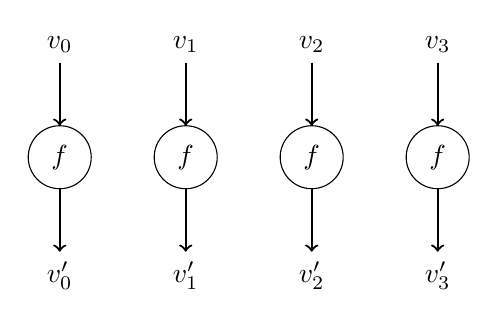
\begin{tikzpicture}[scale=0.8]
\foreach \c in {0,1,2,3} {
    \draw[->,thick] (2*\c+0.5,2) -- (2*\c+0.5,1);
    \draw[->,thick] (2*\c+0.5,0) -- (2*\c+0.5,-1);
    \draw (2*\c+0.5,0.5) circle (0.5);
    \draw (2*\c+0.5,0.5) node { $f$ };
    \draw (2*\c+0.5,2) node[above] { $v_\c$ };
    \draw (2*\c+0.5,-1) node[below] { $v'_\c$ };
}
\end{tikzpicture}
\caption{Structural interpretation of \ensuremath{\Varid{map}}} \label{fig:map}
\end{figure}

\begin{figure}[H]
\centering
\footnotesize
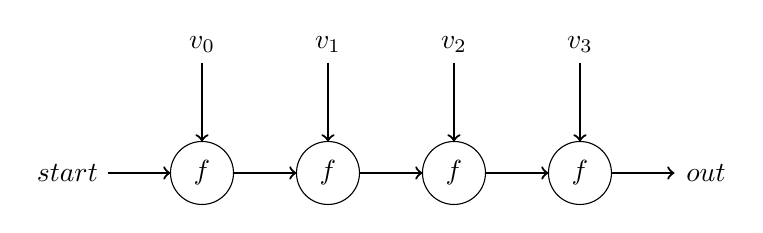
\begin{tikzpicture}[scale=0.8]
\draw (-0.25,-1.5) node[left] { $start$ };
\draw[->,thick] (-0.25,-1.5) -- (0.75,-1.5);
\foreach \c in {0,1,2,3} {
    \draw (2*\c+1.25,0.25) node[above] { $v_\c$ };
    \draw[->,thick] (2*\c+1.25,0.25) -- (2*\c+1.25,-1);
    \draw (2*\c+1.25,-1.5) node { $f$ };
    \draw (2*\c+1.25,-1.5) circle (0.5);
    \draw[->,thick] (2*\c+1.75,-1.5) -- (2*\c+2.75,-1.5);
}
\draw (9.25,-1.5) node { $out$ };
\end{tikzpicture}
\caption{Structural interpretation of \ensuremath{\Varid{vfoldr}}} \label{fig:fold}
\end{figure}

\begin{figure}[H]
\centering
\footnotesize
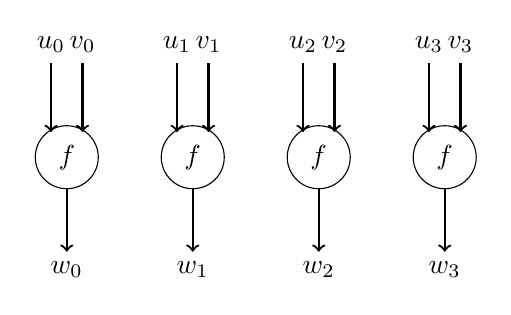
\begin{tikzpicture}[scale=0.8]
\foreach \c in {0,1,2,3} {
    \draw[->,thick] (2*\c+0.25,2) -- (2*\c+0.25,0.9);
    \draw[->,thick] (2*\c+0.75,2) -- (2*\c+0.75,0.9);
    \draw[->,thick] (2*\c+0.5,0) -- (2*\c+0.5,-1);
    \draw (2*\c+0.5,0.5) circle (0.5);
    \draw (2*\c+0.5,0.5) node { $f$ };
    \draw (2*\c+0.25,2) node[above] { $u_\c$ };
    \draw (2*\c+0.75,2) node[above] { $v_\c$ };
    \draw (2*\c+0.5,-1) node[below] { $w_\c$ };
}
\end{tikzpicture}
\caption{Structural interpretation of \ensuremath{\Varid{zipWith}}} \label{fig:zipWith}
\end{figure}

With most important features of \gls{clash} explained we can now introduce the Lustre language, after which we will compare \gls{clash} to it.

\section{Lustre}
The Lustre\cite{halbwachs1991synchronous} language is not used solely as a hardware description language.
It is used for modelling and code generation for safety critical systems.
Even though an extension in the form of Pollux\cite{rocheteau1994pollux} exists to generate hardware from these descriptions, we focus on the Lustre language itself, as more material is available to base a comparison to \gls{clash} on.
Moreover, we do not focus on the process of hardware generation, but merely on the semantical value of descriptions themselves.
Lustre was chosen as it has a number of interesting features which make it a natural match for hardware description languages, such as being synchronous and data-flow oriented.
It also allows decompositional design through nodes.

As explored in the previous section, the synchronous approach works well to create an abstract notion of time and can be used in combination with functional languages. 
Data-flow\cite{ackerman1982data} within Lustre is considered a high level programming language which enables modelling of systems using flows of data which are transformed by nodes in the flow network.
According to \citeauthor{halbwachs1991synchronous} the combination of a synchronous model and data flow languages was not investigated before, but the Lustre language combined the two by ``proposing primitives and structures which restrict data flow systems to only those which can be implemented as bounded memory automata-like programs''\cite{halbwachs1991synchronous}.

\subsection{Data representation}
Within Lustre, data is represented in the form of a \textit{flow}, which is a pair made of
\begin{itemize}
 \item A possibly infinite sequence of values of a given type;
 \item A clock, which represents the instances of time when values exist (c.q. are valid)
\end{itemize}

Since Lustre is a synchronous language, values of the clock do not correspond to any real moments in time but to abstract moments in time. 
Lustre tries to model cyclic behaviour and allows operations to directly act on flows.
From the entire program description and operations on flows the basic clock can be derived, from which all other clocks in the system can be derived. 
The basic clock is simply the smallest possible distinction between two moments in time. 
Temporal operators may be used to create slower clocks, which will be explained shortly.

When defining operations on data, Lustre always acts on the entire flow of data, e.g given a flow \ensuremath{\Conid{X}} and \ensuremath{\Conid{Y}}, the following equation:\\

\begin{changemargin}{1cm}{0cm}
\begin{expansionno}{text only}
\ensuremath{\Conid{Z}\mathrel{=}\Conid{X}\mathbin{+}\Conid{Y}}
\end{expansionno}
\end{changemargin}

is equal to\\
\begin{changemargin}{1cm}{0cm}
\begin{expansionno}{text only}
$\forall n \in \mathbb{N}_0. z_n = x_n + y_n$
\end{expansionno}
\end{changemargin}
, with $n$ being instances of time where both $x$ and $y$ exist. 

\subsection{Temporal operators}
Besides having basic arithmetic operations on flows such as addition and multiplication, Lustre also has a number of temporal operations which specifically modify flows without operating directly on the data of a flow:
\begin{itemize}
\item
    The temporal operator \ensuremath{\textbf{pre}}, shown below, allows us to define basic recursion. \\
    %\begin{texexptitled}[text only,float]{The $pre$ operation in Lustre}{code:lustrepre}

    \begin{changemargin}{1cm}{0cm}
    \begin{expansionno}{text only}
    \ensuremath{\Varid{y}\mathrel{=}\textbf{pre}\;(\Varid{x})}
    \end{expansionno} 
    \end{changemargin}% \\
    %\end{texexptitled}

    This would define a new flow, named $y$, which is simply the right shifted version of $x$. 
    This also means $y_0$, the 0\textsuperscript{th} value of the flow $y$, would have no valid value. 
    Invalid values or values which have no real value are called $nil$ within Lustre.
    The resulting flow would be \\

    \begin{changemargin}{1cm}{0cm}
    \begin{expansionno}{text only}
    $y = (nil,x_0,x_0,x_1,\ldots,x_n)$.
    \end{expansionno}
    \end{changemargin}% \\

\item
    To avoid $nil$ values regular values can be injected into the start of a flow through using the \ensuremath{\to } operator, demonstrated below.\\
    %\begin{texexptitled}[text only,float]{The $\to$ operation in Lustre}{code:lustreto}

    \begin{changemargin}{1cm}{0cm}
    \begin{expansionno}{text only}
    \ensuremath{\Varid{y}\mathrel{=}\mathrm{0}\to (\Varid{x}\mathbin{+}\textbf{pre}\;(\Varid{y}))}
    \end{expansionno}
    \end{changemargin}% \\

    This defines a flow named $y$, with $y_0$ having value $0$ and with every subsequent value being the sum of $x$ until that moment.
    The resulting flow would be \\

    \begin{changemargin}{1cm}{0cm}
    \begin{expansionno}{text only} 
    $y = (0,x_0,x_0+x_1,\ldots,\sum_{0}^{n} x_n)$.
    \end{expansionno}
    \end{changemargin}% \\

\item 
    Lustre also supports multiple clockrates through different operators, such as the \ensuremath{\textbf{when}} operator.
    The \ensuremath{\textbf{when}} operator maps a flow of booleans to a flow of values, sampling only the values on moments when the boolean flow is $true$. 
    The code below shows the mapping of the flow \ensuremath{\Varid{x}} to a clock which is twice as slow as the previous clock.\\

    \begin{changemargin}{1cm}{0cm}
    \begin{expansionno}{text only} 
    \ensuremath{\Varid{b}\mathrel{=}\Varid{true}\to (\neg \;\textbf{pre}\;(\Varid{b}))}\\
    \ensuremath{\Varid{y}\mathrel{=}\Varid{x}\;\textbf{when}\;\Varid{b}}
    \end{expansionno}
    \end{changemargin}% \\

    This defines a flow $b$ with values $(b_0,b_1,\ldots,b_n) = (true,false,true,...)$ and transforms $(x_0,x_1,\ldots,x_n)$ to $(x_0,x_2,\ldots,x_n)$ with a clock which is twice as slow as the basic clock.
\item 
    Upsampling is also possible with the exception of upsampling the basic clock. The \ensuremath{\textbf{current}} operator interpolates a flow of values to a flow of boolean values with a clock faster than its own.
    For instance, taking the flow $x = (x_0,x_2,\ldots,x_n)$ like above, applying it to the flow $(true,true,\ldots,true)$ gives a flow with values: $(x_0,x_0,x_2,x_2,\ldots,x_n,x_n)$.
\end{itemize}

\subsection{Program structure}
Of course, only being able to define expressions using the statements introduced in the previous subsection is not very useful for larger projects. 
To decompose functionality, Lustre introduces the concept of ``nodes''.
Within Lustre a flow network is a composition of nodes, in which nodes may be reused.
Code snippet \ref{code:lustrenode} shows the basic definition of a node.

\begin{texexptitled}[text only,float]{Node definition in Lustre}{code:lustrenode}
\begin{hscode}\SaveRestoreHook
\column{B}{@{}>{\hspre}l<{\hspost}@{}}%
\column{5}{@{}>{\hspre}l<{\hspost}@{}}%
\column{E}{@{}>{\hspre}l<{\hspost}@{}}%
\>[B]{}\textbf{node}\;\Conid{COUNTER}\;(\Varid{x},\Varid{y}\mathbin{:}\Varid{int};\Varid{reset}\mathbin{:}\Varid{bool})\;\Varid{returns}\;(\Varid{s},\Varid{t}\mathbin{:}\Varid{int});{}\<[E]%
\\
\>[B]{}\mathbf{let}{}\<[E]%
\\
\>[B]{}\hsindent{5}{}\<[5]%
\>[5]{}\Varid{s}\mathrel{=}\mathrm{0}\to \mathbf{if}\;\Varid{reset}\;\mathbf{then}\;\mathrm{0}\;\mathbf{else}\;\textbf{pre}\;(\Varid{s})\mathbin{+}\Varid{x}\mathbin{+}\Varid{y};{}\<[E]%
\\
\>[B]{}\hsindent{5}{}\<[5]%
\>[5]{}\Varid{t}\mathrel{=}\mathrm{0}\to \textbf{pre}\;(\Varid{t})\mathbin{+}\Varid{x}\mathbin{+}\Varid{y};{}\<[E]%
\\
\>[B]{}\textbf{tel}{}\<[E]%
\ColumnHook
\end{hscode}\resethooks
\end{texexptitled}

In the description two outputs are defined, \ensuremath{\Varid{s}} and \ensuremath{\Varid{t}}. The \ensuremath{\Varid{t}} output is defined as a sum of the previous value of \ensuremath{\Varid{t}}, combined with the addition of \ensuremath{\Varid{x}} and \ensuremath{\Varid{y}}.
The output \ensuremath{\Varid{s}} is defined to be \ensuremath{\mathrm{0}} when the reset input is toggled, otherwise it will sum the previous value of \ensuremath{\Varid{s}} together with \ensuremath{\Varid{x}} and \ensuremath{\Varid{y}}. 
In this example \ensuremath{\Varid{s}} represents a partial summation, while \ensuremath{\Varid{t}} represents a total summation.

Reusing nodes is also straightforward, as it is much like function application. 
For instance, the node from code snippet \ref{code:lustrereuse} uses the $COUNTER$ from before to sum three consecutive sums of $x$ and $y$ and the total sum. 
In that example the reset is switched every three cycles, while \ensuremath{\Varid{x}} and \ensuremath{\Varid{y}} are summed in \ensuremath{\Varid{s}} only when the reset is \ensuremath{\Varid{false}}.

\begin{texexptitled}[text only,float]{Node reusing in Lustre}{code:lustrereuse}
\begin{hscode}\SaveRestoreHook
\column{B}{@{}>{\hspre}l<{\hspost}@{}}%
\column{5}{@{}>{\hspre}l<{\hspost}@{}}%
\column{11}{@{}>{\hspre}l<{\hspost}@{}}%
\column{E}{@{}>{\hspre}l<{\hspost}@{}}%
\>[B]{}\textbf{node}\;\Conid{SUM3}\;(\Varid{x},\Varid{y}\mathbin{:}\Varid{int})\;\Varid{returns}\;(\Varid{s},\Varid{t}\mathbin{:}\Varid{int});{}\<[E]%
\\
\>[B]{}\mathbf{let}{}\<[E]%
\\
\>[B]{}\hsindent{5}{}\<[5]%
\>[5]{}\Varid{rst}{}\<[11]%
\>[11]{}\mathrel{=}\mathrm{0}\to \mathbf{if}\;(\textbf{pre}\;(\Varid{rst})\mathrel{=}\mathrm{5})\;\mathbf{then}\;\mathrm{0}\;\mathbf{else}\;\textbf{pre}\;(\Varid{rst})\mathbin{+}\mathrm{1};{}\<[E]%
\\
\>[B]{}\hsindent{5}{}\<[5]%
\>[5]{}(\Varid{s},\Varid{t})\mathrel{=}\Conid{COUNTER}\;(\Varid{x},\Varid{y},\Varid{rst}\langle\mathrm{3});{}\<[E]%
\\
\>[B]{}\textbf{tel}{}\<[E]%
\ColumnHook
\end{hscode}\resethooks
\end{texexptitled}

\FloatBarrier
From observing code snippet \ref{code:lustrereuse} we can conclude the following:
\begin{enumerate}
\item  it would be nice to have integer references to previous points in time, so we would be able to write something as\\

\begin{changemargin}{1cm}{0cm}
\begin{expansionno}{text only}
\ensuremath{\Varid{rst}\mathrel{=}\Varid{repeat}\;\mathrm{3}\;\Varid{true}\to (\neg \;\textbf{pre}\;(\mathrm{3},\Varid{rst}))}
\end{expansionno}
\end{changemargin}% \\

, which is a lot clearer and to the point.
The \ensuremath{\Varid{repeat}} operation would then result into a flow $(true,true,true,nil,nil,\ldots,nil)$, after which \ensuremath{\neg \;\textbf{pre}\;(\mathrm{3},\Varid{rst})} defines the remaining cyclic behaviour by generating the next three values as the inverse of the last known value of the flow.
\item Compositions of nodes only show the inputs and outputs of the composition. As a result, when composing nodes, the original definitions of the nodes have to be consulted to reason about the behaviour of the composition. 
\end{enumerate}

Lustre also allows assertions for runtime verification and code generation optimization. 
For instance the assertion \\
\begin{changemargin}{1cm}{0cm}
\begin{expansionno}{text only}
\ensuremath{\textbf{assert}\;\neg \;(\Varid{x}\;\Varid{and}\;\Varid{y});}
\end{expansionno}
\end{changemargin}

will trigger a run-time assertion error if $x$ and $y$ are both true. 
Lustre will also use this to help with code generation, though details on how this is done are not listed.
While run-time assertions are nice to have, for critical applications it is not desirable to merely have error signalling without error handling.
This is especially the case in the context hardware architectures where performance is required.

\subsection{Arrays and recursion}
To allow high-level constructs arrays were introduced to Lustre at version 4. 
Basically these work like vectors in \gls{clash} and \gls{vhdl}.
The sizes of these types have to be known at compile-time, as Lustre simply expands each array depending on how many elements it has. 
This is not really a problem, unless one wants to reuse a design and parameterization is required, as Lustre does not support it.

\citeauthor{halbwachs1993tutorial} show\cite{halbwachs1993tutorial} some examples and details concerning array syntax, which we will briefly repeat here.
For instance, code snippet \ref{code:lustreripple} shows a ripple carry adder using an array of four full adders.
\begin{texexptitled}[text only,float]{Ripple carry adder in Lustre}{code:lustreripple}
\begin{hscode}\SaveRestoreHook
\column{B}{@{}>{\hspre}l<{\hspost}@{}}%
\column{5}{@{}>{\hspre}l<{\hspost}@{}}%
\column{13}{@{}>{\hspre}l<{\hspost}@{}}%
\column{25}{@{}>{\hspre}l<{\hspost}@{}}%
\column{E}{@{}>{\hspre}l<{\hspost}@{}}%
\>[B]{}\textbf{node}\;\Conid{ADD1}\;(\Varid{a},\Varid{b},c_i\mathbin{:}\Varid{bool})\;\Varid{returns}\;(\Varid{s},c_o\mathbin{:}\Varid{bool});{}\<[E]%
\\
\>[B]{}\mathbf{let}{}\<[E]%
\\
\>[B]{}\hsindent{5}{}\<[5]%
\>[5]{}\Varid{s}{}\<[13]%
\>[13]{}\mathrel{=}\Varid{a}\;\Varid{xor}\;\Varid{b}\;\Varid{xor}\;c_i;{}\<[E]%
\\
\>[B]{}\hsindent{5}{}\<[5]%
\>[5]{}c_o{}\<[13]%
\>[13]{}\mathrel{=}(\Varid{a}\;\Varid{and}\;\Varid{b})\;\Varid{or}\;(\Varid{b}\;\Varid{and}\;c_i)\;\Varid{or}\;(c_i\;\Varid{and}\;\Varid{a});{}\<[E]%
\\
\>[B]{}\textbf{tel}{}\<[E]%
\\[\blanklineskip]%
\>[B]{}\textbf{node}\;\Conid{ADD4}\;(\Conid{A},\Conid{B}\mathbin{:}\Varid{bool}^\mathrm{4})\;\Varid{returns}\;(\Conid{S}\mathbin{:}\Varid{bool}^\mathrm{4},\Varid{carry}\mathbin{:}\Varid{bool}){}\<[E]%
\\
\>[B]{}\Varid{var}\;\Conid{C}\mathbin{:}\Varid{bool}^\mathrm{4};{}\<[E]%
\\
\>[B]{}\mathbf{let}{}\<[E]%
\\
\>[B]{}\hsindent{5}{}\<[5]%
\>[5]{}(\Conid{S}\;[\mskip1.5mu \mathrm{0}\mskip1.5mu],\Conid{C}\;[\mskip1.5mu \mathrm{0}\mskip1.5mu]){}\<[25]%
\>[25]{}\mathrel{=}\Conid{ADD1}\;(\Conid{A}\;[\mskip1.5mu \mathrm{0}\mskip1.5mu],\Conid{B}\;[\mskip1.5mu \mathrm{0}\mskip1.5mu],\Varid{false}){}\<[E]%
\\
\>[B]{}\hsindent{5}{}\<[5]%
\>[5]{}(\Conid{S}\;[\mskip1.5mu \mathrm{1}\mathinner{\ldotp\ldotp}\mathrm{3}\mskip1.5mu],\Conid{C}\;[\mskip1.5mu \mathrm{1}\mathinner{\ldotp\ldotp}\mathrm{3}\mskip1.5mu]){}\<[25]%
\>[25]{}\mathrel{=}\Conid{ADD1}\;(\Conid{A}\;[\mskip1.5mu \mathrm{1}\mathinner{\ldotp\ldotp}\mathrm{3}\mskip1.5mu],\Conid{B}\;[\mskip1.5mu \mathrm{1}\mathinner{\ldotp\ldotp}\mathrm{3}\mskip1.5mu],\Conid{C}\;[\mskip1.5mu \mathrm{1}\mathinner{\ldotp\ldotp}\mathrm{3}\mskip1.5mu]);{}\<[E]%
\\
\>[B]{}\hsindent{5}{}\<[5]%
\>[5]{}\Varid{carry}{}\<[25]%
\>[25]{}\mathrel{=}\Conid{C}\;[\mskip1.5mu \mathrm{3}\mskip1.5mu];{}\<[E]%
\\
\>[B]{}\textbf{tel}{}\<[E]%
\ColumnHook
\end{hscode}\resethooks
\end{texexptitled}

The $ADD1$ node is a straightforward implementation of a full adder, which is then used in the ripple carry definition. 
The ripple carry is less straightforward, especially the second equation as it applies an array to a node which only accepts single flows, not arrays of flows.
Lustre allows this sort of behavior, as the compiler can reason about definitions such as these since it only uses compile-time size definitions. 
\citeauthor{halbwachs1993tutorial} call\cite{halbwachs1993tutorial} this polymorphism, but since this does not allow any length of arrays to be used, it is a limited kind of polymorphism. 

Lustre only supports a very specific kind of recursion which is based on being able to determine when the recursion terminates at compile-time.
This is related to totality in programming, a practice where partial functions are not allowed.
Partial functions are undefined for a subset of their domain, which is needed to support general recursion.
Recursion in Lustre is defined by a function which has a certain number of inputs and one constant which is know at compile-time. 
This constant needs to be part of the terminating condition and is needed to unroll the recursion at compile-time.
Code snippet \ref{code:lustrerec} shows the basic principle.

\begin{texexptitled}[text only,float]{Halting recursion in Lustre}{code:lustrerec}
\begin{hscode}\SaveRestoreHook
\column{B}{@{}>{\hspre}l<{\hspost}@{}}%
\column{5}{@{}>{\hspre}l<{\hspost}@{}}%
\column{7}{@{}>{\hspre}l<{\hspost}@{}}%
\column{E}{@{}>{\hspre}l<{\hspost}@{}}%
\>[B]{}\textbf{node}\;\Conid{REC}\;(\Varid{const}\;\Varid{x}\mathbin{:}\Varid{int};\Varid{y}\mathbin{:}\Varid{int})\;\Varid{returns}\;(\Varid{z}\mathbin{:}\Varid{int}){}\<[E]%
\\
\>[B]{}\mathbf{let}{}\<[E]%
\\
\>[B]{}\hsindent{5}{}\<[5]%
\>[5]{}\textbf{with}\;\Varid{x}\mathrel{=}\mathrm{0}{}\<[E]%
\\
\>[5]{}\hsindent{2}{}\<[7]%
\>[7]{}\mathbf{then}\;\Varid{y}{}\<[E]%
\\
\>[5]{}\hsindent{2}{}\<[7]%
\>[7]{}\mathbf{else}\;\Varid{y}\mathbin{+}\Conid{REC}\;(\Varid{x}\mathbin{-}\mathrm{1},\Varid{y});{}\<[E]%
\\
\>[B]{}\textbf{tel}{}\<[E]%
\ColumnHook
\end{hscode}\resethooks
\end{texexptitled}

The above code simply multiplies one input with the other by using the plus operator, e.g. rewriting multiplication as a series of addition.
It is important that \ensuremath{\Varid{x}} is a constant value here, that is, there is one value which \ensuremath{\Varid{x}} represents, and this value may not change during the process defined in this node.
Since this is a constant value it is known at compile-time and as such can be used to unroll the recursion.

We can also define a recurrence relation which captures the essence of recursion.
A sequence of the natural numbers can be defined using the $\rightarrow$ and \ensuremath{\textbf{pre}} operators:\\
\begin{changemargin}{1cm}{0cm}
\begin{expansionno}{text only}
\ensuremath{\Varid{c}\mathrel{=}\mathrm{0}\to \textbf{pre}\;(\Varid{c})\mathbin{+}\mathrm{1};}.
\end{expansionno}
\end{changemargin}

\subsection{Comparison of C$\lambda$aSH and Lustre}
With the basic concepts of both \gls{clash} as Lustre explained we can now compare the two languages.
At first glance both languages seem to have little in common, as Lustre is not really a hardware description language, even though it can be used to model hardware.
However, we can look at its syntax and paradigm and compare those.

Lustre is built around flows, making distinct moments in time explicit. 
It also allows us to refer to previous values of a flow and as such is a stream-based approach.
This can be considered a more behavioural approach when compared to \gls{clash}.
Within \gls{clash} one would have to explicitly store and move values around to achieve the same effect as Lustre, as shown in code snippet \ref{code:clash3cons}, as \gls{clash} is a structural language where we name wires or values.
\begin{texexptitled}[text only,float]{Sum of the last three consecutive values in \gls{clash}}{code:clash3cons}
\begin{hscode}\SaveRestoreHook
\column{B}{@{}>{\hspre}l<{\hspost}@{}}%
\column{5}{@{}>{\hspre}l<{\hspost}@{}}%
\column{9}{@{}>{\hspre}l<{\hspost}@{}}%
\column{E}{@{}>{\hspre}l<{\hspost}@{}}%
\>[B]{}\Varid{add3}\mathbin{::}(\Conid{Int},\Conid{Int})\to \Conid{Int}\to ((\Conid{Int},\Conid{Int}),\Conid{Int}){}\<[E]%
\\
\>[B]{}\Varid{add3}\;(\Varid{s1},\Varid{s2})\;\Varid{i}\mathrel{=}((\Varid{s1'},\Varid{s2'}),\Varid{o}){}\<[E]%
\\
\>[B]{}\hsindent{5}{}\<[5]%
\>[5]{}\mathbf{where}{}\<[E]%
\\
\>[5]{}\hsindent{4}{}\<[9]%
\>[9]{}\Varid{s1'}\mathrel{=}\Varid{i}{}\<[E]%
\\
\>[5]{}\hsindent{4}{}\<[9]%
\>[9]{}\Varid{s2'}\mathrel{=}\Varid{s1}{}\<[E]%
\\
\>[5]{}\hsindent{4}{}\<[9]%
\>[9]{}\Varid{o}\mathrel{=}\Varid{i}\mathbin{+}\Varid{s1}\mathbin{+}\Varid{s2}{}\<[E]%
\ColumnHook
\end{hscode}\resethooks
\end{texexptitled}

Of course, there are also alternatives, such as constructing a single register and using arrow notation to combine two of these into a final component. 
This does not increase the readability however, as it is hard to keep track of how values are used.
The structural approach makes it easy to reason about the resulting hardware representation, yet it is hard to discern what the structure is from this piece of code.

Lustre's syntax makes this more concise, as shown in code snippet \ref{code:lustre3cons}, though the lack of relative indexing of flows is still not very elegant.
The Lustre code is more concise and actually explains how $add3$ should behave in time relative to a certain point, where the \gls{clash} code is still about manipulating values and ``where'' they should go.

\begin{texexptitled}[text only,float]{Sum of the last three consecutive values in Lustre}{code:lustre3cons}
\begin{hscode}\SaveRestoreHook
\column{B}{@{}>{\hspre}l<{\hspost}@{}}%
\column{5}{@{}>{\hspre}l<{\hspost}@{}}%
\column{E}{@{}>{\hspre}l<{\hspost}@{}}%
\>[B]{}\textbf{node}\;\Conid{ADD3}\;(\Varid{i}\mathbin{:}\Varid{int})\;\Varid{returns}\;(\Varid{o}\mathbin{:}\Varid{int});{}\<[E]%
\\
\>[B]{}\mathbf{let}{}\<[E]%
\\
\>[B]{}\hsindent{5}{}\<[5]%
\>[5]{}\Varid{o}\mathrel{=}\textbf{pre}\;(\Varid{i})\mathbin{+}\textbf{pre}\;(\textbf{pre}\;(\Varid{i}))\mathbin{+}\Varid{i};{}\<[E]%
\\
\>[B]{}\textbf{tel}{}\<[E]%
\ColumnHook
\end{hscode}\resethooks
\end{texexptitled}

Aside from the flow aspect, Lustre also offers multiple clocks, although all of these are assumed to be synchronized. 
The same could be implemented in \gls{clash}, although support for this is currently not available. 
The \ensuremath{\textbf{when}} and \ensuremath{\textbf{current}} statements make it easy to upsample or downsample a given clock, which is not implemented concisely in \gls{clash} in its current state.

Of course, \gls{clash} is a language which is specifically designed for hardware description, while Lustre only allow hardware generation through Pollux.
Even so, Lustre gives some nice insights into state, especially how state can be considered a temporal phenomenon. 
Lustre can easily do this because, while it does not allow cyclic definitions entirely, it does allow cycles when a \ensuremath{\textbf{pre}} operator is present. 
A description such as \\
\begin{changemargin}{1cm}{0cm}
\begin{expansionno}{text only}
\ensuremath{\Varid{x}\mathrel{=}\mathrm{0}\to \textbf{pre}\;(\Varid{x})\mathbin{+}\textbf{pre}\;(\Varid{x});}
\end{expansionno}
\end{changemargin}
would not be possible in \gls{clash} without using some form of flow or a state machine which represents such a flow.
It is unfair however to view Lustre's recursive definitions as superior to \gls{clash}'s arrow-based components, as it is perfectly possible to define sequential logic in \gls{clash}. 
However, as \gls{clash} is a functional language, a more ``pure'' recursive specification would be preferable, which is exactly what Lustre offers.

Additionally, both Lustre and \gls{clash} allow bounded vectors or arrays. 
In Lustre it is very easy to create slices, also known as subvectors, from vectors, while it remains a bit cumbersome in \gls{clash}, due to the nature of the host language Haskell.

However, one major advantage \gls{clash} has over Lustre is the type system.
Since \gls{clash} allows type inference, it is possible for a designer to query the type system; the type system can aid the designer.
Type inference allows the compiler to derive types from the structure of expressions themselves.
In Lustre, when an error is encountered it is hard to find out exactly what went wrong, as the Lustre verification only points us in the right direction. 
It never concisely points out what the actual error is.
In \gls{clash} the verification \textit{is} the type system, and as such provides the programmer with a hands-on tool to interface with the compiler, leading to a reduction in time spent to find bugs or faulty logic.



\section{ForSyDe}
The \gls{forsyde}\cite{sander2004system} language, like \gls{clash}, uses the language Haskell to provide a new language te develop embedded systems.
At first the language was focussed on simply modelling systems in general and simulating the descriptions using the \gls{ghc} interpreter. 
With the addition of \gls{vhdl} generation\cite{acosta2007hardware} it became a language in which one can model and synthesize hardware descriptions.
The hardware description capabilities are the parts which this section will focus on.

\gls{forsyde} is a language which currently only supports synchronous systems, approach used by many other hardware description languages as well.
Many hardware description languages use a synchronous model of time as it is relatively simple to simulate. 
It also is an easy model from the designer's perspective.
\gls{forsyde}, unlike \gls{clash}, uses the \gls{edsl} approach to avoid the effort needed to create a compiler, type-checker, et cetera from scratch.
A \gls{dsl} is, as its name implies, a language designed specifically with one domain in mind.
A \gls{edsl} however, is a specific kind of \gls{dsl}, which uses a host language in which the guest language is \tif{embedded}.
Embedding a language has some advantages, like using existing syntax, tools of the host language, and not needing to develop an entire compiler from scratch. 
The \gls{edsl} approach does not offer many advantages over the leveraging approach used by \gls{clash}, a property which will be discussed later in more detail.
For now it is enough to know that leveraging binds a language to a specific \textit{implementation}, while the \gls{edsl} approach binds a language to a specific \textit{language}.
In practice \gls{ghc} is the defacto standard compiler for Haskell, and as such there is not much difference in dependence on either the language or the specific implementation.

\subsection{Processes}
Within ForSyDe, systems are modelled using an abstraction called processes. 
These processes can be combined through networks. 
This approach is very similar to data-flow approaches discussed before.
Perhaps unsurprisingly, \gls{forsyde} uses Haskell's list structure to represent signals.
A process can then be seen as a function which transforms one signal to another signal.
However, as functions operate on entire signals, it is harder for a compiler to discern what \textit{elements} of the signal are used.
This makes it harder to do optimalizations based on these descriptions, since functions which are referential transparent with regards to the elements of a signal offer many ways to optimize code, a quality which is often associated with Haskell.

The fact that signals are needed in \gls{forsyde} can be seen in how processes are defined.
\gls{forsyde} supplies a number of process constructors which take a function as input, an approach often used in Haskell. 
First, they define a signal in the style of lists with \ensuremath{\coloneq} as the Signal constructor
\begin{changemargin}{1cm}{0cm}
\begin{expansionno}{text only}
\ensuremath{\mathbf{data}\;\Conid{Signal}\;\Varid{a}\mathrel{=}\Varid{a}\coloneq\Conid{Signal}\;\Varid{a}}
\ensuremath{| \Conid{NullS}}
\end{expansionno}
\end{changemargin}
, which is used in the definition of the \ensuremath{\Varid{mapSY}} constructor, shown by code snippet \ref{code:formapsy}.

\begin{texexptitled}[text only,float]{The \ensuremath{\Varid{mapSY}} process constructor in \gls{forsyde}}{code:formapsy}
\begin{hscode}\SaveRestoreHook
\column{B}{@{}>{\hspre}l<{\hspost}@{}}%
\column{17}{@{}>{\hspre}l<{\hspost}@{}}%
\column{E}{@{}>{\hspre}l<{\hspost}@{}}%
\>[B]{}\Varid{mapSY}\mathbin{::}(\Varid{a}\to \Varid{b})\to \Conid{Signal}\;\Varid{a}\to \Conid{Signal}\;\Varid{b}{}\<[E]%
\\
\>[B]{}\Varid{mapSY}\;\anonymous \;\Conid{NullS}{}\<[17]%
\>[17]{}\mathrel{=}\Conid{NullS}{}\<[E]%
\\
\>[B]{}\Varid{mapSY}\;\Varid{f}\;(\Varid{x}\coloneq\Varid{xs})\mathrel{=}\Varid{f}\;\Varid{x}\coloneq(\Varid{mapSY}\;\Varid{f}\;\Varid{xs}){}\<[E]%
\ColumnHook
\end{hscode}\resethooks
\end{texexptitled}
The process resulting from \ensuremath{\Varid{mapSY}} clearly behaves the same as a regular \ensuremath{\Varid{map}} function over lists as is commonly used in Haskell.

Aside from \ensuremath{\Varid{mapSY}}, \gls{forsyde} also supplies the following process constructors:
\begin{itemize}
 \item \ensuremath{\Varid{zipWithSY}}, which is analogous to \ensuremath{\Varid{zipWith}} from Haskell; it takes two \ensuremath{\Conid{Signal}}s and uses a function to combine these \ensuremath{\Conid{Signal}}s into one.
\item \textit{delaySY$_k$}, which delays a \ensuremath{\Conid{Signal}} with $k$ discrete time steps. It can be used to create feedback, for instance to create the \ensuremath{\Varid{sourceSY}} constructor.
\item \ensuremath{\Varid{sourceSY}}, which generates an infinite series of outputs.
\item \ensuremath{\Varid{scanlSY}}, which acts much like the the \ensuremath{\Varid{scanl}} of Haskell. 
When thinking of streams it makes sense to use \ensuremath{\Varid{scanl}} to encapsulate state. 
A stream of values together with a function which acts on two individual elements of the stream can then be used to `store' intermediate results. 
Of course, since these intermediate results only depend on the previous values of the Signal and the function applied to it it is still a pure function. 
\item \ensuremath{\Varid{mooreSY}}, a constructor for a Moore machine; a process from which the output only depends on the internal state.
\item \ensuremath{\Varid{mealySY}}, a constructor for a Mealy machine; a process from which the output depends on both the internal state and the input signals.
\item \ensuremath{\Varid{unzipSY}}, which is analogous to the \ensuremath{\Varid{unzip}} function in Haskell. 
\end{itemize}

These process constructors can be composed to create new, more complex processes, as in code snippet \ref{code:formulacc}.
\begin{texexptitled}[text only,float]{Stateful multiply-accumulate in \gls{forsyde}}{code:formulacc}
\begin{hscode}\SaveRestoreHook
\column{B}{@{}>{\hspre}l<{\hspost}@{}}%
\column{5}{@{}>{\hspre}l<{\hspost}@{}}%
\column{9}{@{}>{\hspre}l<{\hspost}@{}}%
\column{E}{@{}>{\hspre}l<{\hspost}@{}}%
\>[B]{}\Varid{macSY}\mathbin{::}\Conid{Num}\;\Varid{a}\Rightarrow \Conid{Signal}\;\Varid{a}\to \Conid{Signal}\;\Varid{a}\to \Conid{Signal}\;\Varid{a}{}\<[E]%
\\
\>[B]{}\Varid{macSY}\;\Varid{x}\;\Varid{y}\mathrel{=}\Varid{scanlSY}\;(\mathbin{+})\;\mathrm{0}\;\Varid{prod}{}\<[E]%
\\
\>[B]{}\hsindent{5}{}\<[5]%
\>[5]{}\mathbf{where}{}\<[E]%
\\
\>[5]{}\hsindent{4}{}\<[9]%
\>[9]{}\Varid{prod}\mathrel{=}\Varid{zipWithSY}\;(\mathbin{*})\;\Varid{x}\;\Varid{y}{}\<[E]%
\ColumnHook
\end{hscode}\resethooks
\end{texexptitled}

This is equivalent to the following Haskell code using lists:
\begin{changemargin}{1cm}{0cm}
\begin{expansionno}{text only}
\ensuremath{\Varid{mac}\;\Varid{xs}\;\Varid{ys}\mathrel{=}\Varid{scanl}\;(\mathbin{+})\;\mathrm{0}\;(\Varid{zipWith}\;(\mathbin{*})\;\Varid{xs}\;\Varid{ys})}
\end{expansionno}
\end{changemargin}
\citeauthor{sander2004system} list\cite{sander2004system} more detailed examples, but this example should be enough to explain the principle.

\subsection{Deep and shallow embedding}
While not mentioned before, the only way to generate \gls{vhdl} from a \gls{forsyde} model is to use the so-called ``deeply embedded'' approach. 
The regular \gls{forsyde} model does not contain the information needed to generate \gls{vhdl} code.
This is due to the fact the language is embedded in the host language.
Since it is embedded in the host language, it is restricted by the host language as well.
This restriction has certain downsides, as one would normally not be able to \tif{observe sharing} within a certain program, functionality which is needed to detect cycles in a program.
Cycles are often needed in hardware descriptions to describe feedback, so observable sharing is necessary.
Fortunately Lava\cite{claessen2002embedded,bjesse1998lava} faced the same problems at an earlier stage and solved this through observable sharing\cite{claessen1999observable}.

In order to use this a non-backwards compatible change had to be made, which is referred to as the ``deeply embedded'' approach. 
This approach heavily depends on using Template Haskell, which makes the \gls{ast} of the program c.q. hardware description accessible from within the language itself.
The usage of Template Haskell introduces several problems, which will be looked at in detail in the comparison with \gls{clash}.
The gist of it is however that to use functionality many Haskell programmers take for granted, such as polymorphism and higher order functions, functions that depend on them need to have a specific type signature.
These functions must then be passed into Quasi-Quatation\cite{sheard2002template} blocks, all of which only hinder readability and do nothing to aid the designer.

\subsection{Program structure}
To provide more structure to the hardware design, the designer has the ability to define circuit definitions using hierachical structures. 
These structures have a strong relation with the structures used in \gls{vhdl}, probably both for reasons of familiarity as well as ease of translation. 
\gls{forsyde} supplies the following hierachical structures:
\begin{itemize}
\item 
A \ensuremath{\Conid{Port}} is almost identical to \gls{vhdl}'s port clause, aside from the fact that in \gls{forsyde} it is not allowed to mix input and output ports; two separate ports have to be made per system, provided they indeed have both in and output ports. 
The port structure serves as an interface between the outside world and the system. 
However, there wasn't a lot of concrete information available as to what the actual use of this structure is. 
Since it is so closely related to \gls{vhdl} it seems natural to use these interfaces to mix regular \gls{vhdl} code with generated \gls{vhdl} code. 
These ports are named \ensuremath{\Conid{InPort}} and \ensuremath{\Conid{OutPort}} and consist of a list of tuples containing the name and the type of each input or output.
\item A \ensuremath{\Conid{Circuit}} is defined as a function which transforms an \ensuremath{\Conid{InPort}} to an \ensuremath{\Conid{OutPort}}. The circuit definition then simply consists of applying functions to the specific input ports of the circuit.
\item The circuits defined can then be turned into a \ensuremath{\Conid{Block}}, which is a white-box which can not be connected directly to other system structures. A \ensuremath{\Conid{Block}} can be instantiated, or transformed into a \ensuremath{\Conid{BlockIns}} structure.
This structure is a black-box, but its inputs and outputs can be used to connect to other parts of the system. 
A \ensuremath{\Conid{Block}} and \ensuremath{\Conid{BlockIns}} are similar to entity-architecture pairs and component in \gls{vhdl}. 
\end{itemize}

\subsection{Arrays and Vectors}
Vectors in \gls{clash} are not much different from those used in \gls{forsyde} as the library introduced\cite{acosta2008forsyde} by \citeauthor{acosta2008forsyde} was used as an inspiration for \gls{clash} as mentioned in ``Clash: From Haskell to Hardware''\cite{clashchris}.
As such it is not very interesting to go into details, as any comparison will simply state they are very similar and offer the same advantages and disadvantages. 
We already discussed the advantages and disadvantages of this approach in the context of \gls{clash} in a previous section.

\subsection{Comparison of C$\lambda$aSH and ForSyDe}
\gls{clash} and \gls{forsyde} seem to have a lot in common. 
They both use Haskell, albeit in different ways.
The methods used to translate the model is different, as well as the model itself and the way this model is presented to the designer.

\gls{forsyde} is a language which makes streaming explicit and allows the designer to create processes which act on these streams.
\gls{clash} on the other hand does not deal with streams at all and is more structural in its approach, allowing the designer to define a circuit in terms of \tif{wires} or \tif{individual values}, not in \textit{streams} of values. 
\gls{clash} is able to describe a circuit structurally because it is able to transform a program description from the outside of the language it is created in.
This is not the case for \gls{forsyde}, as it can only analyze whatever the language Haskell and its \gls{ghc} implementation allow it to analyze. 

As mentioned before, \gls{clash} leverages Haskell and as such is bound tightly to a specific implementation of \gls{ghc}.
In \gls{clash} the translation is done outside the programming environment of Haskell, so it can look from the outside in and has access to Haskell's Core language to transform definitions from the Haskell source straight to \gls{vhdl}.
This is different from the \gls{forsyde} approach, which uses Template Haskell to access the \gls{ast} of the program from within the limits of the language it is embedded in.
This limits on the translation of \tif{user defined} descriptions:
\begin{itemize}
 \item When defining a function and passing it to a process constructor the number of parameters must equal the number of arguments; currying is not allowed.
 \item The signature of the function supplied to the process constructor has to be made explicit, regardless of the function.
 \item Pattern matching is limited to literals, variables and wildcards; no pattern matching on data constructors is allowed.
 \item \ensuremath{\mathbf{where}} and \ensuremath{\mathbf{let}} clauses are not allowed.
 \item Polymorphism is only supported for instances of a certain typeclass. 
 In ``Hardware Synthesis in ForSyDe''\cite{acosta2007hardware} it is mentioned it was only possible for \ensuremath{\Conid{Int}} and \ensuremath{\Conid{Bool}} at the time, with options to expand it. 
 Nevertheless, it still makes polymorphism less clear since it changes the type for for instance the \ensuremath{\Varid{mapSY}} from 
 %\begin{texexptitled}[text only,float]{|mapSY| and |hdMapSY| in \gls{forsyde}}{code:forhdmap}
\begin{changemargin}{1cm}{0cm}
\begin{expansionno}{text only}
\ensuremath{\Varid{mapSY}\mathbin{::}(\Varid{a}\to \Varid{b})\to \Conid{Signal}\;\Varid{a}\to \Conid{Signal}\;\Varid{b}}
\end{expansionno}
\end{changemargin}
 to
\begin{changemargin}{1cm}{0cm}
\begin{expansionno}{text only}
\ensuremath{\Varid{hdMapSY}\mathbin{::}(\Conid{HDPrimType}\;\Varid{a},\Conid{HDPrimType}\;\Varid{b})\Rightarrow \Conid{HDFun}\;(\Varid{a}\to \Varid{b})\to \Conid{HDSignal}\;\Varid{a}\to \Conid{HDSignal}\;\Varid{b}}.
\end{expansionno}
\end{changemargin}
The details of this notation are not that important, as they are only needed by the underlying system to enable transformation to \gls{vhdl}.

 \item Passing a function to a process constructor requires the use of Template Haskell.
\end{itemize}

Most of these limitations are quite severe when considering how these features are used in Haskell itself.
Not having \ensuremath{\mathbf{where}} or \ensuremath{\mathbf{let}} clauses is undesirable, since it is considered idiomatic Haskell. 
The same could be said for currying, except the value of currying depends on what the semantics of currying are in the context of hardware description languages. 
Within \gls{clash} currying is used for parameterization, something which seems natural at first, but might benefit from a more strict separation between parameters and inputs.
One of the bigger issues is the use of Template Haskell and Quasi Quotation.
Quasi Quotation is a shorthand method to \tif{splice} existing code into Haskell at compile-time. 
A full overview of Quasi Quotation is out of the scope of this study, but giving an example will most likely clear up any misconceptions.

To show how this influences the syntax we can define a simple component which just adds one to its input, as shown in code snippet \ref{code:hdplus1}.
\begin{texexptitled}[text only,float]{Definition of hdPlus1 in \gls{forsyde}}{code:hdplus1}
\begin{hscode}\SaveRestoreHook
\column{B}{@{}>{\hspre}l<{\hspost}@{}}%
\column{5}{@{}>{\hspre}l<{\hspost}@{}}%
\column{37}{@{}>{\hspre}l<{\hspost}@{}}%
\column{61}{@{}>{\hspre}l<{\hspost}@{}}%
\column{E}{@{}>{\hspre}l<{\hspost}@{}}%
\>[B]{}\Varid{hdPlus1}\mathbin{::}\Conid{HDSignal}\;\Conid{Int}\to \Conid{HDSignal}\;\Conid{Int}{}\<[E]%
\\
\>[B]{}\Varid{hdPlus1}\mathrel{=}\Varid{hdMapSY}\;\Varid{doPlus1}{}\<[E]%
\\
\>[B]{}\hsindent{5}{}\<[5]%
\>[5]{}\mathbf{where}\;\Varid{doPlus1}\mathrel{=}\mathbin{\$}(\Varid{mkHDFun}\;[\mskip1.5mu \Varid{d}\mid {}\<[37]%
\>[37]{}\Varid{doPlus1}\mathbin{::}\Conid{Int}\to \Conid{Int}{}\<[E]%
\\
\>[37]{}\Varid{doPlus1}\;\Varid{a}\mathrel{=}\Varid{a}\mathbin{+}\mathrm{1}{}\<[61]%
\>[61]{}\mid \mskip1.5mu]){}\<[E]%
\ColumnHook
\end{hscode}\resethooks
\end{texexptitled}

The definition of \ensuremath{\Varid{doPlus1}} consists of a splicing ( \tif{\$()} ) operation and a Quasi Quotation operation ( $[d \mid \: \mid ]$).
The Quasi Quotation operation takes the definition of the function, extracts its \gls{ast} at compile-time, and the splicing operation injects it in the proper point, also at compile-time.
There are some downsides with this approach, which make it not really suited for a hardware description language.

Firstly, it can give uninformative error messages when there is an error in the definition of the function which is being spliced into code, or when there is an type error between two Template Haskell code fragments, although this has been greatly improved in recent \gls{ghc} versions.
Secondly, it makes it harder to inspect program elements from the interpreter, as the quoted part has the type $Q Exp$ when evaluated in the interpreter. 
Thirdly, and most importantly, it adds extra syntax for no apparent reason, at least as far as the hardware designer is concerned. 
Without knowing why these Quasi Quotations exists, which would be common as it is considered advanced Haskell, it will be very hard to ignore all this syntactic `noise'.
While the reasoning given is clear, it will make it harder for a designer to adopt this language. 

The \gls{clash} implementation is much simpler in comparison and, with this simplicity in mind, can be both interpreted as a structural representation, naming the \tif{wires}, or a behavioral implementation, naming the \tif{values}:\\
\begin{changemargin}{1cm}{0cm}
\begin{expansionno}{text only}
\ensuremath{\Varid{plus1}\;\Varid{x}\mathrel{=}\Varid{x}\mathbin{+}\mathrm{1}}.
\end{expansionno}
\end{changemargin}

Of course one can get by without even naming anything due to partial application and \tif{point-free}\footnote{Point-free programming refers to the practice of not mentioning the arguments in a function definition. It is used when composing functions without actually labelling the data} programming through a simple $plus1 = (+1)$.

\section{Conclusion}
After discussing the various languages we can conclude that each of these languages have their advantages and disadvantages.
\gls{clash} offers a seemingly seamless translation of Haskell to \gls{vhdl} when the idiomatic style of Haskell is preferred.
This is the major downside of the \gls{forsyde} approach, which cannot use common features as pattern matching, top-level type inference and other features considered idiomatic Haskell.
The fact that it depends on Quasi-Quotation and Template Haskell is also a downside in that, for the uninitiated at least, it is not clear \textit{why} the splicing and quotation operations are needed.

Unlike Lustre, \gls{forsyde} and \gls{clash} do not offer protection against errors in synchronization. 
While Lustre does not have a type system like Haskell-based languages, it at least offers the ability to verify whether synchronization and composition behaves as expected.
The downside of this approach is that it is stream-based, which may make it harder for hardware designers to reason about circuits without developing a feeling for the system first.
The fact that it was not developed with hardware in mind does not help, as it never tries to relate its concepts to the concepts hardware designers are familiar with.

While \gls{forsyde} has the power of the type system, it does nothing to exploit it. 
The type system in \gls{forsyde} mainly serves as a tool of limitation pertaining to making the model work in Haskell, not a tool of limitation to aid the developer in actually creating hardware descriptions.
Lustre has such a tool, but does not give the developer the hands-on it requires to actually have it aid development. There, it is only used as a tool for catching errors.

Like \gls{forsyde}, Lustre takes the streaming approach. 
From a hardware perspective this is not desirable, as it does not match well with the mental model most hardware designers have.

While sequences of values are important for how execution of computations behave, generally designers want to decompose a problem, solve the decomposed problems and compose solutions.
With sequences of values the compositions of solutions may influence each other, with effects of these compositions largely unclear or hidden in the specific structure of expressions.

As a result, it appears that \gls{clash} has a more intuitive and simple model of expression, even though it does not handle state as elegantly as its counterparts.
\gls{clash} does have the advantage of flexibility due to its leveraging approach, making it easier to introduce specific features which could make its type system more helpful in aiding the designer with hardware design.
